\documentclass[12pt,a4paper]{article}
\usepackage[utf8]{inputenc}
\usepackage[T1]{fontenc}
\usepackage{geometry}
\usepackage{titlesec}
\usepackage{hyperref}
\usepackage{graphicx}
\usepackage{fancyhdr}
\usepackage{enumitem}
\usepackage{tabularx}
\usepackage{longtable}
\usepackage{float}
\usepackage{pdflscape}
\geometry{left=2.5cm,right=2.5cm,top=2.5cm,bottom=2.5cm}
\setlength{\headheight}{15pt}

\pagestyle{fancy}
\fancyhf{}
\fancyhead[L]{S-007: Renewal \& Upsell Advisor}
\fancyhead[R]{Selected Sections}
\fancyfoot[C]{\thepage}

\title{\textbf{Software Requirements Specification}\\ \vspace{1cm} \Large Renewal \& Upsell Advisor\\ \vspace{0.5cm} \large Selected Sections}
\author{}
\date{Version: 1.0\\ December 28, 2025}

\begin{document}

\maketitle
\thispagestyle{empty}
\begin{center}
    \textbf{Confidential}
\end{center}

\newpage

\tableofcontents

\newpage

\section{Scope}

\subsection{In-Scope}
\begin{itemize}
    \item \textbf{Renewal Risk Management:}
    \begin{itemize}
        \item Contract expiration tracking and automated alerts
        \item Multi-factor churn prediction using ML models
        \item Customer health scoring based on usage, engagement, and sentiment
        \item Risk segmentation (High, Medium, Low) with confidence scores
    \end{itemize}
    \item \textbf{Upsell \& Cross-sell Intelligence:}
    \begin{itemize}
        \item Product adoption and feature usage analysis
        \item Revenue expansion opportunity identification
        \item Cross-sell recommendations based on customer profile and behavior
        \item Whitespace analysis for untapped product offerings
    \end{itemize}
    \item \textbf{Automated Playbook Recommendations:}
    \begin{itemize}
        \item Personalized renewal and expansion plays
        \item Multi-channel outreach cadence suggestions (Email, Phone, Meeting)
        \item Value messaging templates tailored to customer pain points and outcomes
        \item Best-action recommendations with success probability scores
    \end{itemize}
    \item \textbf{Integration Capabilities:}
    \begin{itemize}
        \item Primary: Salesforce CRM, Stripe/Chargebee billing platforms, Google Analytics/Mixpanel
        \item Secondary: Customer Success platforms (Gainsight, ChurnZero), Email (Gmail, Outlook), Product analytics tools
        \item Webhook-based real-time data synchronization
    \end{itemize}
    \item \textbf{Analytics \& Reporting:}
    \begin{itemize}
        \item Renewal forecast dashboard with ARR projections
        \item Pipeline health metrics and trend analysis
        \item Agent performance tracking and recommendation outcomes
        \item Executive summary reports with KPI visualization
    \end{itemize}
\end{itemize}

\subsection{Out-of-Scope}
\begin{itemize}
    \item Contract negotiation and legal document generation
    \item Direct payment processing and transaction handling
    \item Customer onboarding and implementation workflows
    \item Product roadmap planning and feature prioritization
    \item Marketing campaign creation and execution
    \item Technical support ticket management
    \item Full financial accounting and revenue recognition
    \item Integration with non-B2B SaaS business models (e.g., e-commerce, retail)
    \item Manual override of contract terms or pricing
    \item Real-time voice call monitoring and transcription
\end{itemize}

\section{Functional Requirements}

\subsection{FR-1: Contract \& Renewal Tracking}
\subsubsection{FR-1.1: Contract Data Ingestion}
\begin{itemize}
    \item System SHALL ingest contract data from Salesforce including: contract ID, account name, ARR/MRR, start date, end date, renewal date, contract terms
    \item System SHALL automatically sync contract updates within 5 minutes of changes in source system
    \item System SHALL support bulk import of historical contract data (minimum 5 years)
\end{itemize}
\subsubsection{FR-1.2: Renewal Timeline Monitoring}
\begin{itemize}
    \item System SHALL track all contracts with renewal dates within 90-day window
    \item System SHALL automatically create renewal opportunity records in Salesforce 90 days before expiration
    \item System SHALL categorize renewals by time horizon: Immediate (0-30 days), Near-term (31-60 days), Future (61-90 days)
\end{itemize}

\subsection{FR-2: Churn Risk Prediction}
\subsubsection{FR-2.1: Risk Scoring Model}
\begin{itemize}
    \item System SHALL calculate renewal risk score (0-100) for each account using ML model
    \item Risk score SHALL incorporate features: product usage (login frequency, feature adoption), support metrics (ticket volume, resolution time), payment history (late payments, failed charges), engagement (email opens, meeting attendance), sentiment (NPS, survey responses)
    \item System SHALL update risk scores daily via batch processing
    \item System SHALL provide 85\% prediction accuracy (validated on historical data)
\end{itemize}
\subsubsection{FR-2.2: Risk Segmentation}
\begin{itemize}
    \item System SHALL classify accounts into risk categories:
    \begin{itemize}
        \item High Risk: Score 70-100 (churn probability >50\%)
        \item Medium Risk: Score 40-69 (churn probability 25-50\%)
        \item Low Risk: Score 0-39 (churn probability <25\%)
    \end{itemize}
    \item System SHALL display top 5 risk factors for each account
    \item System SHALL provide confidence intervals for predictions
\end{itemize}
\subsubsection{FR-2.3: Early Warning Alerts}
\begin{itemize}
    \item System SHALL send real-time alerts when account moves to High Risk category
    \item Alerts SHALL include: account name, ARR at risk, risk score, primary risk factors, recommended actions
    \item System SHALL support alert routing rules (assign to CSM, AE, or team lead based on account ownership)
\end{itemize}

\subsection{FR-3: Upsell \& Cross-sell Identification}
\subsubsection{FR-3.1: Expansion Opportunity Detection}
\begin{itemize}
    \item System SHALL identify upsell opportunities based on:
    \begin{itemize}
        \item User license utilization (threshold: >80\% of purchased seats)
        \item Feature usage patterns (high engagement with premium features on basic plan)
        \item API usage limits (approaching rate limits)
        \item Storage consumption (exceeding 75\% of allocated quota)
    \end{itemize}
    \item System SHALL calculate expansion revenue potential for each opportunity
    \item System SHALL rank opportunities by expected value and win probability
\end{itemize}
\subsubsection{FR-3.2: Cross-sell Recommendations}
\begin{itemize}
    \item System SHALL recommend complementary products based on:
    \begin{itemize}
        \item Current product usage (collaborative filtering)
        \item Industry segment and company size
        \item Similar customer adoption patterns
    \end{itemize}
    \item System SHALL support whitespace analysis (identify unused products in customer’s plan tier)
\end{itemize}
\subsubsection{FR-3.3: Opportunity Qualification}
\begin{itemize}
    \item System SHALL assign propensity score (0-100) to each upsell opportunity
    \item System SHALL filter opportunities with score >60 for proactive outreach
    \item System SHALL estimate deal size and expected close date
\end{itemize}

\subsection{FR-4: Automated Playbook Recommendations}
\subsubsection{FR-4.1: Playbook Library}
\begin{itemize}
    \item System SHALL include minimum 15 pre-built playbooks:
    \begin{itemize}
        \item Renewal Playbooks: High-Risk Intervention, Executive Business Review, Value Realization Workshop, Competitive Displacement Defense
        \item Upsell Playbooks: License Expansion, Feature Upgrade, Multi-Year Commitment, Premium Support Add-on
    \end{itemize}
    \item Each playbook SHALL contain: trigger conditions, outreach cadence (timeline), email/call script templates, success metrics
\end{itemize}
\subsubsection{FR-4.2: Playbook Matching Engine}
\begin{itemize}
    \item System SHALL automatically recommend playbook based on: account risk level, contract value, industry vertical, customer lifecycle stage
    \item System SHALL support A/B testing of playbook effectiveness
    \item System SHALL allow CSM/AE to override recommendations
\end{itemize}
\subsubsection{FR-4.3: Personalized Messaging}
\begin{itemize}
    \item System SHALL generate personalized email templates with dynamic variables:
    \begin{itemize}
        \item Customer-specific ROI metrics
        \item Recent usage statistics
        \item Relevant case studies from similar companies
        \item Competitive insights (if applicable)
    \end{itemize}
    \item Templates SHALL maintain brand voice and compliance requirements
\end{itemize}

\subsection{FR-5: Outreach Cadence Optimization}
\subsubsection{FR-5.1: Multi-Channel Sequencing}
\begin{itemize}
    \item System SHALL recommend outreach sequence across channels: Email, Phone Call, LinkedIn Message, In-Product Notification
    \item System SHALL optimize timing based on: historical engagement patterns, recipient time zone, industry benchmarks
    \item System SHALL support customizable cadence templates (3-touch, 5-touch, 7-touch sequences)
\end{itemize}
\subsubsection{FR-5.2: Task Automation}
\begin{itemize}
    \item System SHALL automatically create tasks in Salesforce for recommended actions
    \item System SHALL set due dates aligned with playbook timeline
    \item System SHALL send reminders 24 hours before task due date
\end{itemize}

\subsection{FR-6: Sentiment \& Engagement Analysis}
\subsubsection{FR-6.1: Email Sentiment Tracking}
\begin{itemize}
    \item System SHALL analyze sentiment from customer emails using NLP (spaCy, Hugging Face)
    \item System SHALL classify sentiment as Positive, Neutral, Negative with confidence score
    \item System SHALL detect sentiment shifts (declining trend over 30-day window)
\end{itemize}
\subsubsection{FR-6.2: Engagement Monitoring}
\begin{itemize}
    \item System SHALL track engagement metrics: email open rate, link click rate, meeting acceptance rate, response time
    \item System SHALL flag disengaged accounts (no response to 3+ outreach attempts)
\end{itemize}

\subsection{FR-7: Analytics \& Reporting}
\subsubsection{FR-7.1: Renewal Pipeline Dashboard}
\begin{itemize}
    \item Dashboard SHALL display:
    \begin{itemize}
        \item Total ARR at risk (segmented by risk level)
        \item Renewal rate forecast (current quarter, next quarter)
        \item Top 10 at-risk accounts by ARR
        \item Churn reason analysis (historical)
    \end{itemize}
    \item Dashboard SHALL support filtering by: renewal date range, account segment, assigned CSM/AE
\end{itemize}
\subsubsection{FR-7.2: Expansion Revenue Tracking}
\begin{itemize}
    \item Dashboard SHALL display:
    \begin{itemize}
        \item Total expansion pipeline value
        \item Upsell conversion rate
        \item Average deal size by opportunity type
        \item Time-to-close for expansion deals
    \end{itemize}
\end{itemize}
\subsubsection{FR-7.3: Agent Performance Metrics}
\begin{itemize}
    \item System SHALL track:
    \begin{itemize}
        \item Prediction accuracy (renewal outcome vs. predicted risk)
        \item Playbook effectiveness (conversion rate by playbook type)
        \item Alert response time (time from alert to first action)
        \item Revenue saved via early intervention
    \end{itemize}
\end{itemize}
\subsubsection{FR-7.4: Executive Reports}
\begin{itemize}
    \item System SHALL generate weekly executive summary including: ARR retention forecast, Top risks \& mitigations, Expansion opportunities closed, YoY performance trends
    \item Reports SHALL be exportable in PDF and CSV formats
\end{itemize}

\subsection{FR-8: Integration Requirements}
\subsubsection{FR-8.1: Salesforce Integration}
\begin{itemize}
    \item System SHALL sync bidirectionally: Accounts, Opportunities, Contracts, Tasks, Activities
    \item System SHALL support custom Salesforce objects
    \item System SHALL handle API rate limits (5,000 calls/day for Enterprise edition)
\end{itemize}
\subsubsection{FR-8.2: Billing Platform Integration}
\begin{itemize}
    \item System SHALL ingest data from Stripe/Chargebee: Subscription details, Payment history, Plan changes, Failed charges
    \item System SHALL process webhook events in real-time
\end{itemize}
\subsubsection{FR-8.3: Analytics Platform Integration}
\begin{itemize}
    \item System SHALL collect product usage data from: Google Analytics (page views, session duration), Mixpanel (event tracking, funnel analysis), Custom analytics APIs
\end{itemize}

\subsection{FR-9: Notification System}
\subsubsection{FR-9.1: Alert Delivery}
\begin{itemize}
    \item System SHALL support notification channels: Slack (direct message, channel post), Email (digest or real-time), In-app notification center, Microsoft Teams
    \item Users SHALL configure notification preferences per alert type
\end{itemize}
\subsubsection{FR-9.2: Alert Types}
\begin{itemize}
    \item System SHALL generate alerts for:
    \begin{itemize}
        \item High-risk account detection
        \item Upsell opportunity identification
        \item Contract expiration (30/60/90-day reminders)
        \item Failed payment events
        \item Significant usage decline
    \end{itemize}
\end{itemize}

\subsection{FR-10: Security \& Compliance}
\subsubsection{FR-10.1: Authentication \& Authorization}
\begin{itemize}
    \item System SHALL support SSO via OAuth 2.0 (Okta, Azure AD)
    \item System SHALL enforce role-based access control (RBAC): Admin, Sales Manager, CSM, AE, Read-Only
    \item System SHALL log all user actions for audit trail
\end{itemize}
\subsubsection{FR-10.2: Data Privacy}
\begin{itemize}
    \item System SHALL encrypt data at rest (AES-256) and in transit (TLS 1.3)
    \item System SHALL support GDPR/CCPA compliance (data anonymization, deletion)
    \item System SHALL mask sensitive PII in non-production environments
\end{itemize}

\section{Flow Diagram / Architecture Diagram}

\subsection{System Architecture Overview}
The Renewal \& Upsell Advisor follows a microservices architecture with three primary layers:

\begin{figure}[H]
    \centering
    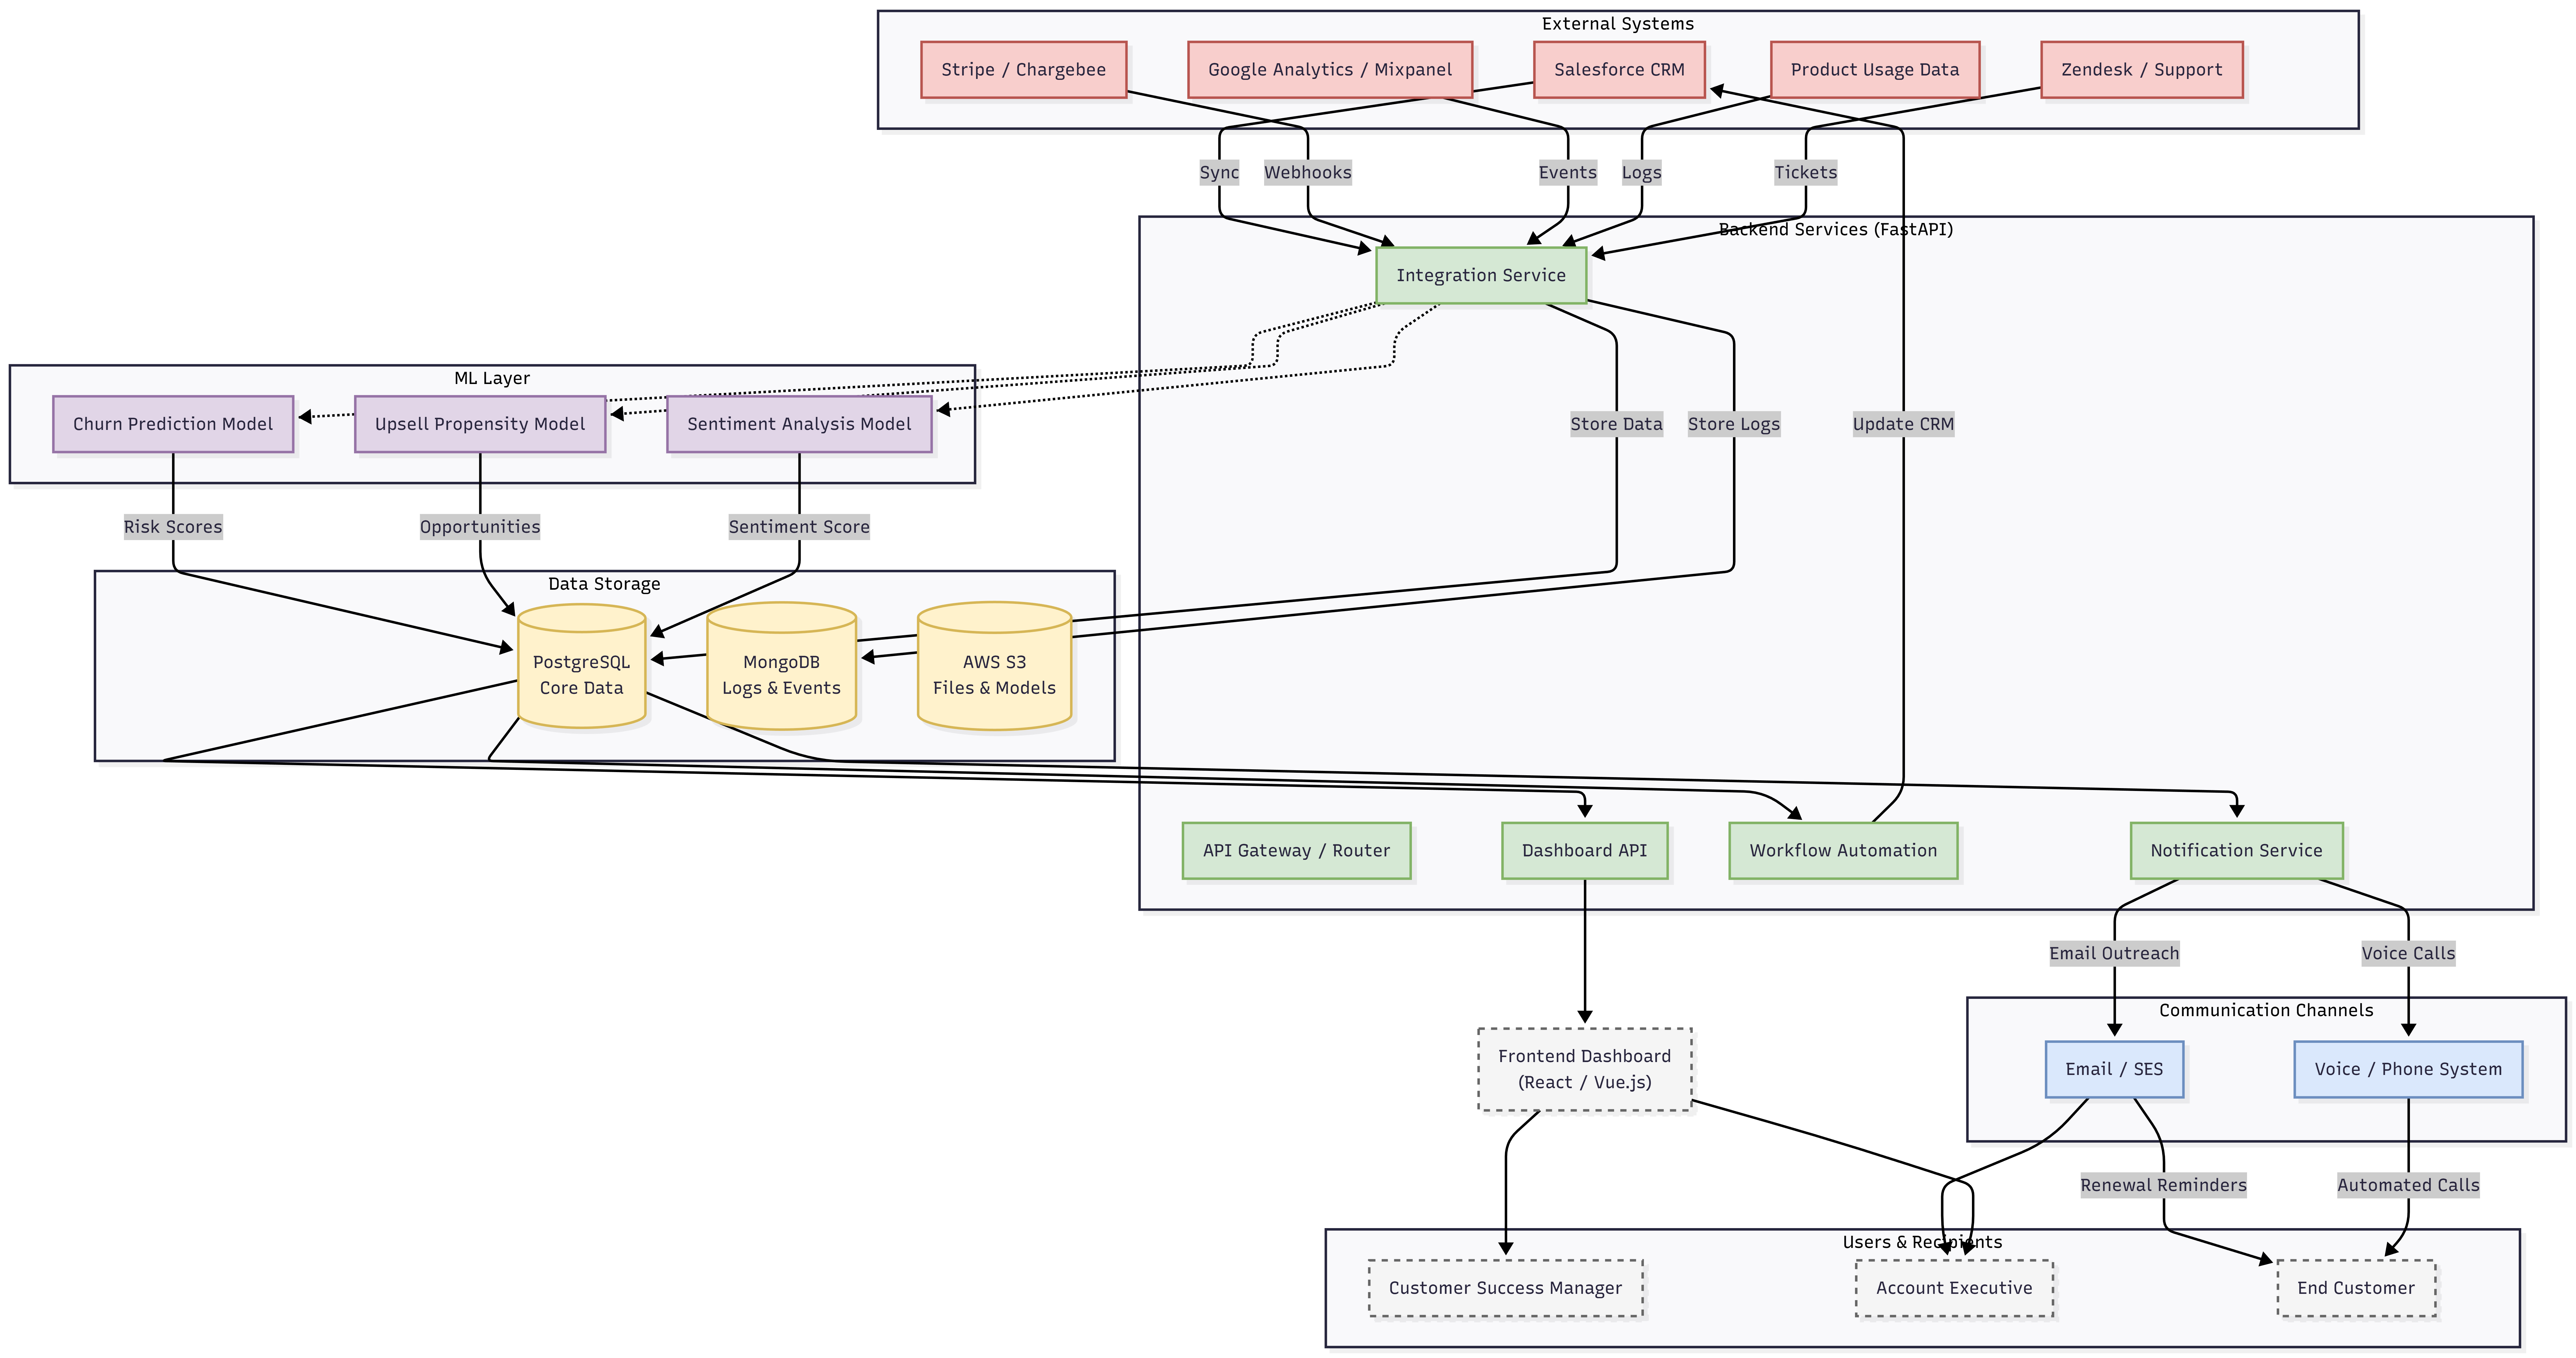
\includegraphics[width=0.9\textwidth]{1.png}
    \caption{System Architecture Diagram - High Level}
\end{figure}

\begin{figure}[H]
    \centering
    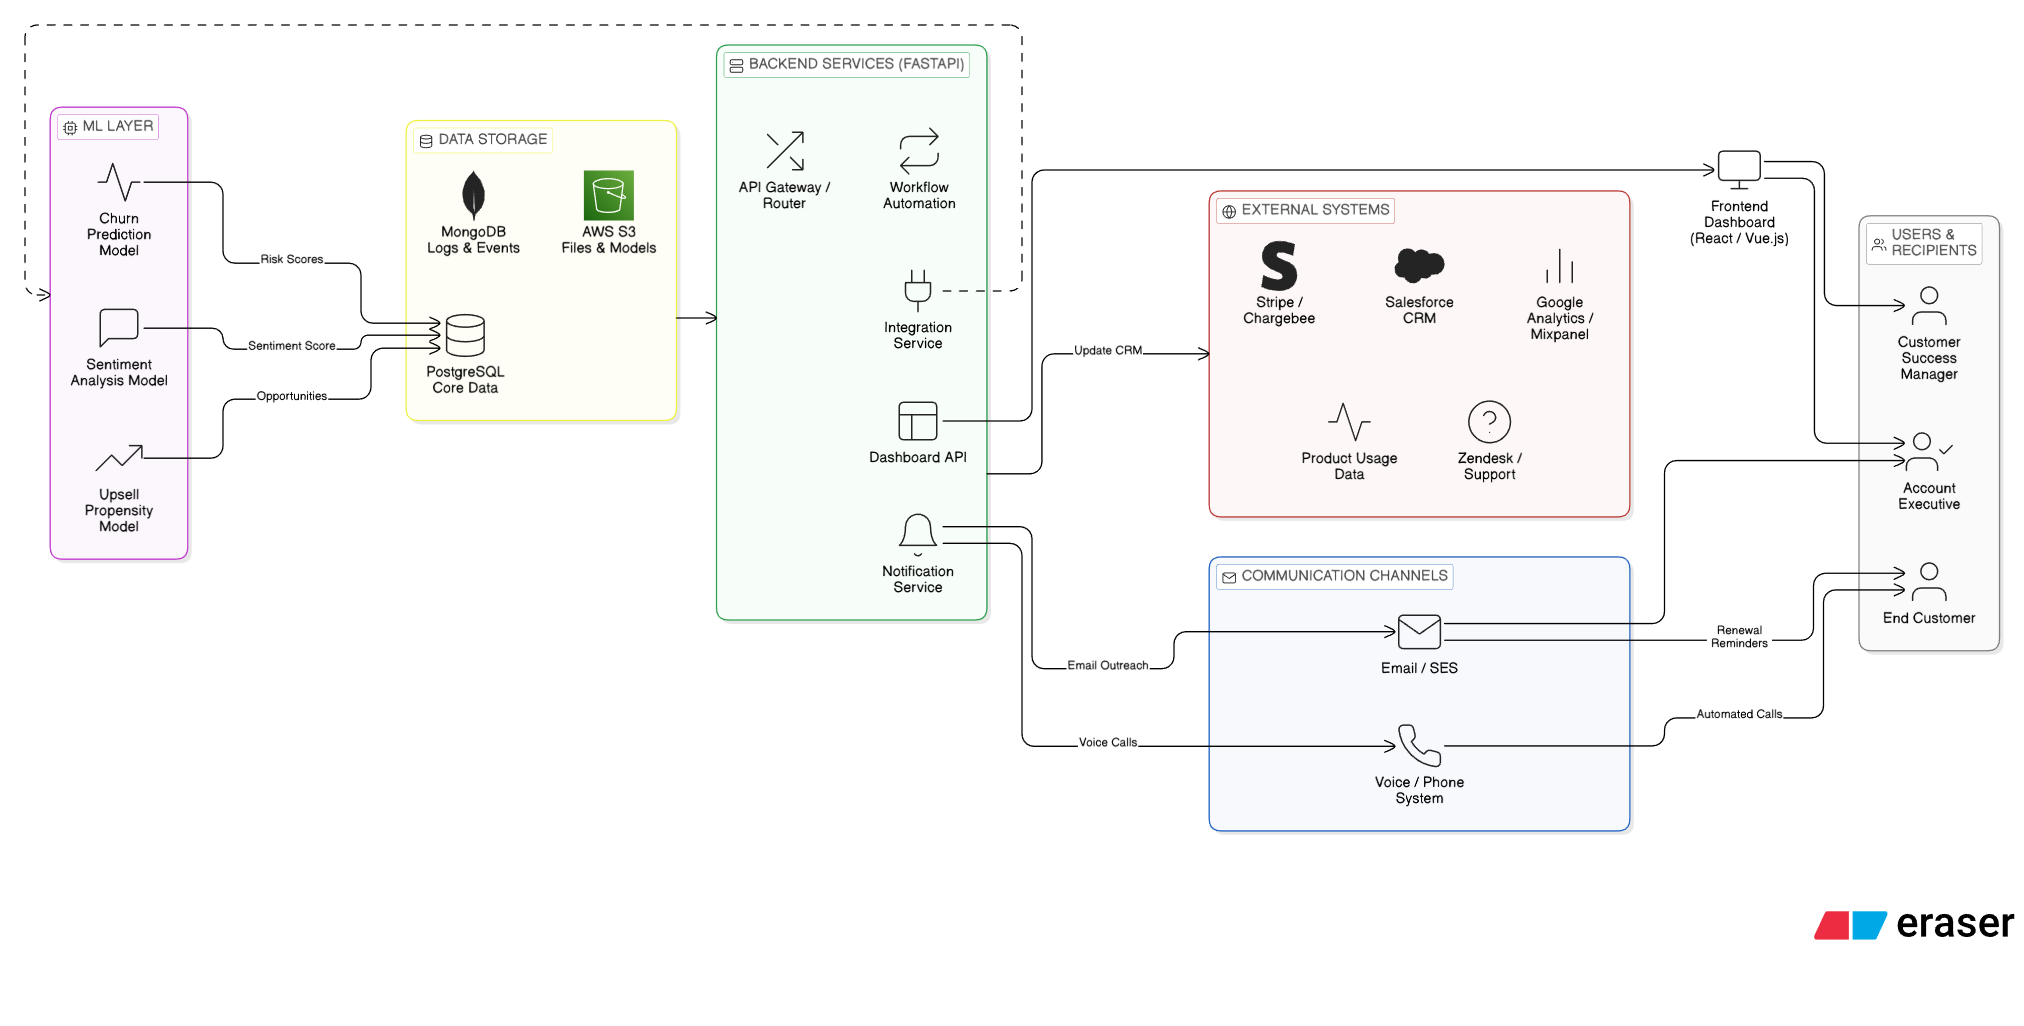
\includegraphics[width=0.9\textwidth]{2.png}
    \caption{System Architecture Diagram - Detailed Data Flow}
\end{figure}

\begin{enumerate}
    \item \textbf{Integration Layer:} Handles bidirectional data synchronization with external systems (Salesforce, Stripe, Analytics platforms)
    \item \textbf{Processing Layer:} Executes data transformation, feature engineering, ML inference, and business logic
    \item \textbf{Presentation Layer:} Provides user interfaces (dashboard) and notification delivery
\end{enumerate}

\subsection{Data Flow}
\textbf{Ingestion Phase:}
\begin{enumerate}
    \item External systems (Salesforce, Stripe, Analytics) push data via webhooks or API polling
    \item Integration Service validates and queues incoming data
    \item ETL Pipeline processes raw data and stores in Data Warehouse
\end{enumerate}

\textbf{Processing Phase:}
\begin{enumerate}
    \item Feature Engineering Service extracts signals from historical data
    \item ML Inference Service calculates risk scores and upsell propensity
    \item Playbook Engine matches accounts to recommended plays
    \item Results stored in PostgreSQL for real-time access
\end{enumerate}

\textbf{Action Phase:}
\begin{enumerate}
    \item Notification Service triggers alerts (Slack, Email) based on threshold rules
    \item Workflow Automation creates tasks/opportunities in Salesforce
    \item Dashboard displays insights and recommendations to users
\end{enumerate}

\subsection{Architecture Components}
\textbf{Microservices:}
\begin{itemize}
    \item Integration Service (Node.js / Python FastAPI)
    \item ETL Pipeline Service (Apache Airflow)
    \item Feature Engineering Service (Python)
    \item ML Inference Service (Python + MLflow)
    \item Playbook Recommendation Engine (Python)
    \item Notification Service (Python + Celery)
    \item Dashboard API (FastAPI)
    \item Frontend Application (React)
\end{itemize}

\textbf{Data Stores:}
\begin{itemize}
    \item PostgreSQL: Contracts, accounts, opportunities, tasks
    \item MongoDB: Event logs, unstructured customer interactions
    \item Redis: Session cache, API response cache, task queue
    \item Snowflake/BigQuery: Historical analytics, reporting
    \item S3: Model artifacts, exported reports
\end{itemize}

\textbf{Supporting Infrastructure:}
\begin{itemize}
    \item API Gateway (Kong / AWS API Gateway): Rate limiting, authentication
    \item Message Queue (RabbitMQ / AWS SQS): Async task processing
    \item Load Balancer (AWS ALB): Traffic distribution
    \item Monitoring Stack (Prometheus + Grafana): Metrics, alerts
\end{itemize}

\subsection{Detailed Flow Descriptions}
\subsubsection{Flow 1: Churn Risk Detection}
\begin{enumerate}
    \item Daily batch job retrieves contracts expiring in 90 days from Salesforce
    \item System fetches associated usage data (Google Analytics), payment history (Stripe), support tickets (Zendesk)
    \item Feature Engineering Service calculates: 30-day login frequency decline, feature adoption rate, NPS score, payment punctuality score
    \item ML Model predicts churn probability for each account
    \item Accounts with risk score >70 trigger High Risk alert
    \item Playbook Engine recommends intervention playbook
    \item Notification sent to assigned CSM via Slack with action items
    \item System creates task in Salesforce: "Schedule Executive Business Review"
\end{enumerate}

\subsubsection{Flow 2: Upsell Opportunity Identification}
\begin{enumerate}
    \item Real-time webhook from product analytics detects: Account XYZ reaches 85\% user license utilization
    \item System retrieves account profile: current plan tier, contract value, renewal date
    \item Upsell Propensity Model calculates expansion likelihood (78\% probability)
    \item System estimates expansion value: +25 seats = \$75K additional ARR
    \item Opportunity automatically created in Salesforce with "Qualified" stage
    \item Personalized email template generated: "Your team is growing fast. Unlock 25 more seats with preferred pricing."
    \item AE receives in-app notification with recommended talk track
    \item System schedules 3-touch follow-up sequence (Email Day 1, Call Day 3, Email Day 7)
\end{enumerate}

\subsubsection{Flow 3: Renewal Forecast Generation}
\begin{enumerate}
    \item Monthly batch job aggregates all renewals for next quarter
    \item System calculates weighted renewal forecast: (Low Risk ARR $\times$ 95\%) + (Medium Risk $\times$ 75\%) + (High Risk $\times$ 40\%)
    \item Expansion pipeline added to base renewal forecast
    \item Historical conversion rates applied to upsell opportunities
    \item Dashboard displays: Total forecasted ARR, Confidence intervals (P10, P50, P90), Risk-adjusted retention rate
    \item Executive report exported to PDF and emailed to VP Sales
\end{enumerate}

\textbf{Note:} Detailed architecture diagram is provided separately as a visual chart. Reference the flow diagram PDF attached with this SRS document.

\section{Competitive Analysis}

\subsection{Market Landscape}
The renewal and upsell intelligence market includes specialized customer success platforms, revenue operations tools, channel automation platforms such as Yagna iQ, and AI-powered sales enablement solutions. Key competitors offer varying degrees of automation, predictive analytics, CPQ capabilities, and CRM/channel integration.

\subsection{Primary Competitors}

\subsubsection{Gainsight Customer Success}
\textbf{Product URL:} \url{https://www.gainsight.com/}

\textbf{Strengths:}
\begin{itemize}
    \item Industry-leading customer health scoring with ML-powered predictions
    \item Native Salesforce integration with deep data synchronization
    \item Comprehensive playbook automation and journey orchestration
    \item Strong analytics and executive reporting dashboards
    \item Extensive third-party integrations (200+ apps)
\end{itemize}

\textbf{Weaknesses:}
\begin{itemize}
    \item Complex setup requiring significant admin resources
    \item Higher cost (enterprise pricing starts at \$50K+/year)
    \item Steeper learning curve for end users
    \item Limited flexibility for mid-market companies
\end{itemize}

\textbf{Technical Approach:} Gainsight uses Bayesian recursive models for churn prediction, combining usage telemetry, support data, and sentiment analysis. Their "Rules Engine" triggers automated workflows based on multi-dimensional health scores. Data aggregation occurs in their proprietary data warehouse with scheduled ETL jobs from source systems.

\subsubsection{ChurnZero}
\textbf{Product URL:} \url{https://churnzero.com/}

\textbf{Strengths:}
\begin{itemize}
    \item Real-time customer engagement tracking and alerts
    \item Easy-to-use interface with faster time-to-value
    \item Strong renewal forecasting with Forecast Hub
    \item AI agents (Vibes, Harbinger, Beacon) for risk and opportunity detection
    \item Competitive pricing for mid-market segment
\end{itemize}

\textbf{Weaknesses:}
\begin{itemize}
    \item Less robust analytics compared to Gainsight
    \item Limited customization for complex enterprise workflows
    \item Fewer native integrations (relies on Zapier for some connections)
    \item Reporting can feel rigid per user feedback
\end{itemize}

\textbf{Technical Approach:} ChurnZero emphasizes real-time event streaming from product analytics. Their AI agents use sentiment shift detection (NLP on emails/chat) and behavioral pattern matching. Renewal forecasting combines health scores with historical win/loss rates. They employ a segment-based approach for playbook recommendations.

\subsubsection{Totango}
\textbf{Product URL:} \url{https://www.totango.com/}

\textbf{Strengths:}
\begin{itemize}
    \item Product adoption-focused with deep usage analytics
    \item Flexible pricing and modular features (scale as needed)
    \item Strong customer segmentation capabilities
    \item Pre-built success plans and templates
    \item Good balance of simplicity and functionality
\end{itemize}

\textbf{Weaknesses:}
\begin{itemize}
    \item Churn prediction less sophisticated than Gainsight
    \item Limited upsell recommendation intelligence
    \item Fewer automated playbook options
    \item Smaller user community and ecosystem
\end{itemize}

\textbf{Technical Approach:} Totango’s core philosophy centers on product usage as the primary health indicator. They auto-generate health scores based on feature adoption patterns without requiring manual configuration. Segments are dynamically updated based on lifecycle stage and account attributes. Renewal risk is inferred from usage decline trends.

\subsubsection{Catalyst (formerly ProsperWorks)}
\textbf{Product URL:} \url{https://www.catalyst.io/}

\textbf{Strengths:}
\begin{itemize}
    \item Unified customer data platform (CDP) approach
    \item Strong revenue forecasting and pipeline management
    \item AI-driven insights with "moments" (trigger events)
    \item Modern UI with intuitive UX
\end{itemize}

\textbf{Weaknesses:}
\begin{itemize}
    \item Relatively new player (smaller customer base)
    \item Fewer proven ML models compared to Gainsight
    \item Limited third-party integration ecosystem
    \item Still building out playbook automation
\end{itemize}

\textbf{Technical Approach:} Catalyst aggregates customer data into a unified profile (CDP model). Their "moments" feature detects trigger events (e.g., usage spike, support escalation) using rule-based and ML hybrid models. Revenue forecasting uses cohort analysis and time-series prediction.

\subsubsection{Yagna iQ Channel Ecosystem Platform}
\textbf{Product URL:} \url{https://www.yagnaiq.com/}

\textbf{Strengths:}
\begin{itemize}
    \item \textbf{High ROI \& Efficiency:} Proven to save 125+ hours per 100 contracts and increase on-time renewal rates by 20--25\%.
    \item \textbf{Zero-Touch Automation:} "Set and forget" workflows for low-value, high-volume renewals, triggering proactive quotes 90/60/30 days in advance.
    \item \textbf{Unified Channel View:} Solves the "1000 Portal Problem" by aggregating multi-vendor data into a single dashboard for distributors and resellers.
    \item \textbf{Security \& Integration:} ISO 27001 certified with native connectors for Salesforce, Microsoft Dynamics, and major ERPs.
\end{itemize}

\textbf{Weaknesses:}
\begin{itemize}
    \item Highly specialized for \textit{indirect} channel sales (Vendors $\rightarrow$ Distributors $\rightarrow$ Resellers), which may be overkill for direct-only SaaS businesses.
    \item UI/UX is function-first (industrial strength) rather than "consumer-grade" aesthetic compared to modern PLG tools.
\end{itemize}

\textbf{Technical Approach:} Yagna iQ operates as a cloud-native "Channel Ecosystem" platform. It ingests "Golden Record" data from vendor ERPs/CRMs and normalizes it for downstream partners. Its core engine uses AI/ML to identify "Smart Leads" for cross-selling (XSUS Cloud) and automates the entire quote-to-cash cycle for renewals (Renewal Cloud) using event-driven triggers.


\subsection{Innovation \& Differentiation Strategy}
\subsubsection{Core Innovation: The "Agentic" Shift}
The primary innovation of our Renewal \& Upsell Advisor is the fundamental shift from \textbf{Passive Analytics} (Dashboards) to \textbf{Active Agency} (Co-Pilots).

\begin{enumerate}
    \item \textbf{From "Insights" to "Actions":}
    Legacy platforms (Gainsight, Yagna iQ) identify a risk and populate a dashboard, requiring a human Key Account Manager (KAM) to log in, interpret the data, and decide on an action.
    \textbf{Our Innovation:} The Agent identifies the risk and \textit{immediately drafts the remedial action} (e.g., a personalized email, a meeting agenda, or a discount offer) for the KAM to approve. The KAM manages \textit{decisions}, not data.

    \item \textbf{Generative vs. Static Playbooks:}
    Competitors use rigid "If-Then" rule engines (e.g., "If health score < 50, send Email Template B").
    \textbf{Our Innovation:} We utilize Large Language Models (LLMs) to generate \textit{context-aware} playbooks on the fly. The Agent reads the last 10 emails, analyzes the support ticket tone, and generates a truly personalized message that acknowledges specific client pain points, rather than using a generic template.

    \item \textbf{Unified "Growth Loop" Architecture:}
    Most platforms treat "Renewals" (Defense) and "Upsells" (Offense) as separate pipelines.
    \textbf{Our Innovation:} We model them as a single \textbf{Revenue Optimization Problem}. Every interaction is scored for both Retention Probability and Expansion Propensity simultaneously. The Agent will suppress an upsell offer if the renewal risk is high, or leverage a successful renewal to immediately pitch an upsell, creating a continuous growth loop.
\end{enumerate}

\subsubsection{Our Competitive Advantages}
\begin{enumerate}
    \item \textbf{Zero-Login Experience:} The Agent lives where the KAM works (Slack, Teams, Email). There is no "platform" to learn or log into.
    \item \textbf{Hyper-Personalization at Scale:} Using Generative AI to craft unique account plans for thousands of long-tail customers that would otherwise receive generic automation.
    \item \textbf{Faster Time-to-Value:} 7-day deployment via API overlay, compared to 6--12 week implementation cycles for heavy platforms like Yagna or Gainsight.
\end{enumerate}

\subsection{Feature Comparison Matrix}

% Use small font for the table to fit the width
\footnotesize
% Reduce padding to maximize space
\setlength{\tabcolsep}{2pt}
% Add some vertical space
\renewcommand{\arraystretch}{1.2}

\begin{longtable}{|p{2.2cm}|p{2.8cm}|p{1.7cm}|p{1.7cm}|p{1.5cm}|p{1.7cm}|p{2.2cm}|}
\hline
\textbf{Feature} & \textbf{Our Agent} & \textbf{Gainsight} & \textbf{ChurnZero} & \textbf{Totango} & \textbf{Catalyst} & \textbf{Yagna iQ} \\
\hline
Churn Prediction & \textbf{Action-Oriented} & Descriptive & Descriptive & Basic & Descriptive & Analytical \\
\hline
Upsell Propensity & \textbf{Generative Pitch} & Partial & Yes & Limited & Yes & Smart Leads \\
\hline
Playbook Engine & \textbf{GenAI (Dynamic)} & Rigid Rules & Rigid Rules & Rigid Rules & Rigid Rules & Rigid Workflow \\
\hline
Real-Time Alerts & \textbf{Drafts Response} & Notification & Notification & No & Notification & Quote Trigger \\
\hline
User Interface & \textbf{Chat/Slack (Headless)} & Dashboard & Dashboard & Dashboard & Dashboard & Portal \\
\hline
Salesforce Sync & \textbf{ bidirectional Agent} & Native Sync & Sync & Sync & Native Sync & Native Sync \\
\hline
Deployment & \textbf{7 Days (Overlay)} & 8--12 weeks & 4--6 weeks & 2--4 weeks & 3--5 weeks & 4--8 weeks \\
\hline
Pricing & \textbf{Usage/Outcome} & Seat-Based & Seat-Based & Seat-Based & Seat-Based & Volume-Based \\
\hline
Core AI Tech & \textbf{LLM + RAG} & Predictive ML & Predictive ML & Basic ML & Predictive ML & Predictive ML \\
\hline
\end{longtable}
\normalsize


\end{document}
